%!/usr/bin/env latex
% espina-user-manual.tex: EspINA user manual
% @Author:      <Jorge Peña> (<jpena@cesvima.upm.es>)
% @Created:     2012-09-17.
% @Last Change: 2012-09-17.
% @Revision:    0.0

\documentclass[a4paper,10pt]{article}

\usepackage{ifpdf}
\usepackage{ifthen}

% D E F I N I C I O N   D E   L A S   C A B E C E R A S   D E   C A P I T U L O S
\usepackage{type1cm}
\usepackage{floatflt}
\usepackage{float}

\ifpdf
  \usepackage{color,graphicx}
  \usepackage[pdftex, % or dvips or dvipsone
  %------------- Backref Switch ---------------------------
  pagebackref,                     % or backref
  %------------- Color Links ------------------------------
  colorlinks=false, %true,
  linkcolor=black, %webbrown,            % defined below
  filecolor=black, %blue,
  citecolor=black, %green,
%------------- Doc Info ---------------------------------
  pdftitle={EspINA User Manual},
  pdfauthor={Jorge Pena Pastor},
  pdfsubject={Reconstruction},
  pdfkeywords={reconstruction, neuroscience, fib},
%------------ Doc View ----------------------------------
bookmarksopen=false
%pdfpagemode=UseOutlines %is the default, use ``None'' otherwise
%hypertexnames=false
]
{hyperref}
  
  %defined in manuscrit.tex
  %\graphicspath{                  % where are the figures?
  %       {pdf/}{jpg/}
  % }
\else
  \usepackage[pagebackref]{hyperref}
  \usepackage{graphicx}
  \usepackage{color}
  %defined in manuscrit.tex
  %\graphicspath{                  % where are the figures?
  %	 {ps/} 
  %}
\fi

\definecolor{MyDarkBlue}{rgb}{0,0.1,0.45}%0,0.08,0.45
\hypersetup{citecolor=MyDarkBlue}

% FONTS
\usepackage[english]{babel}
\usepackage[utf8]{inputenc}
\usepackage[T1]{fontenc}

% MULTICOLUMNS
\usepackage{multicol}

% TABLE
\usepackage{longtable}
\usepackage{supertabular}

% FIGURES
\usepackage{fancybox}
%\usepackage{psfrag} 
\usepackage{subfigure}

% ENUMERATES
\usepackage{mdwlist}


% MATHEMATICS
\usepackage{amsmath,amssymb}
\usepackage{amscd}
\usepackage{amsfonts}
\usepackage{array}
\usepackage{mathrsfs}
\usepackage{textcomp}
\usepackage{latexsym}

% GRAPHISM
\usepackage{graphics}
\usepackage{pst-text} %to place text along curves

% LIST ENVIRONMENTS
\usepackage{enumitem}

% B I B L I O G R A P H I E
\usepackage[colon]{natbib}
% Biblio grafía en el índice
\usepackage{tocbibind} 

% T A B L E   O F   C O N T E N T   F O R   A P P E N D I X
\usepackage{appendix}

% U R L
\usepackage{url}


% PAGE
\usepackage[headings]{fullpage}
\usepackage{placeins}

% C O L O R S
\definecolor{webbrown}{rgb}{.6,0,0}
\definecolor{gris55}{gray}{0.55}
\definecolor{bleu}{rgb}{0,0,0.5}

\ifpdf
  \graphicspath{                  % where are the figures?
	  {fig/}
}
\else
  \graphicspath{                  % where are the figures?
	  {fig/}
}
\fi

% C A B E C E R A S   M O L O N A S
\usepackage{fancyhdr}
\pagestyle{fancy}
\fancyhf{}
\fancyfoot[LO,LE]{
\includegraphics[scale=0.29]{logo-cajal}}
\fancyfoot[CO,CE]{\thepage}
\fancyfoot[RO,RE]{
\includegraphics[scale=0.1]{logo-cesvima}}
\fancyhead[LO,LE]{\textbf{EspINA}}
\fancyhead[RO,RE]{\textbf{Cajal Blue Brain Project}}
\renewcommand{\headrulewidth}{0.5pt}
\renewcommand{\footrulewidth}{0.5pt}

\usepackage{lastpage}
\usepackage{a4wide} 
\usepackage{moreverb}
\usepackage{hangcaption}
\usepackage{listings}

%Formulas
\newcommand{\ela}{\\ \nonumber}
%Probability Definitions
\newcommand{\Pb}[3][]{\ensuremath{\text{P}(#2\mid #3\ \pi_{#1})}}
%\newcommand{\Pb}[3][\pi]{\ensuremath{\text{P}(#2\mid #3\ #1)}}
%\newcommand{\PK}[1]{\ensuremath{\pi_{\text{#1}}}}
%\newcommand{\PK}[1]{\ensuremath{\textit{PK}_{\textit{#1}}}}
\newcommand{\Gauss}[3]{\ensuremath{G_{\mu(\text{#1}),\sigma(\text{#2})}(#3)}}
\newcommand{\Uni}[1]{\ensuremath{\textbf{U}(k_\text{#1})}}
%Variables
%%Prob
\newcommand{\Tool}[3]{
\begin{tabular}{m{0.8cm} m{13cm}}
\frame{\includegraphics[width=0.7cm{#2}} &
\textbf{#1}: #3
\end{tabular}

}
%%Control
\newcommand{\Roll}[1][]{
\ifthenelse{\equal{#1}{}}{\text{Roll}}{[\text{Roll} = #1]}
}
\newcommand{\Pitch}[1][]{
\ifthenelse{\equal{#1}{}}{\text{Pitch}}{[\text{Pitch} = #1]}
}
\newcommand{\Yaw}[1][]{
\ifthenelse{\equal{#1}{}}{\text{Yaw}}{[\text{Yaw} = #1]}
}
\newcommand{\Throttle}{\ensuremath{\delta{\text{Throttle}}}}
%%Sensors
\newcommand{\Sl}[1][]{
\ifthenelse{\equal{#1}{}}
	{
	\ensuremath{\text{Sonar}_\text{L}}
	}
%else
	{
	\ensuremath{[\text{Sonar}_\text{L} = #1]}
	}
}
\newcommand{\Sr}[1][]{
\ifthenelse{\equal{#1}{}}
	{
	\ensuremath{\text{Sonar}_\text{R}}
	}
%else
	{
	\ensuremath{[\text{Sonar}_\text{R} = #1]}
	}
}
\newcommand{\Sf}[1][]{
\ifthenelse{\equal{#1}{}}
	{
	\ensuremath{\text{Sonar}_\text{F}}
	}
%else
	{
	\ensuremath{[\text{Sonar}_\text{F} = #1]}
	}
}
\newcommand{\Sd}[1][]{
\ifthenelse{\equal{#1}{}}
	{
	\ensuremath{\text{Sonar}_\text{D}}
	}
%else
	{
	\ensuremath{[\text{Sonar}_\text{D} = #1]}
	}
}

%%CONSTANTS
\newcommand{\espina}{EspINA}

%%Writing
\newcommand{\ToDo}[1]{\textit{\textbf{ToDo: } #1}}

%P O R T A D A
\author{Jorge PEÑA PASTOR}
\title{\textbf{Esp}ina \textbf{I}nteractive \textbf{N}euron \textbf{A}nalizer}


\begin{document}

\maketitle \clearpage
\tableofcontents \clearpage
%\listoffigures %\clearpage\listoftables


\section{Introduction}

\espina{} is a tool for segmenting, editing and analyzing neuroscientific images acquired using microscopy.
The program is been developed by the CesViMa (Centro de Supercomputación y Visualización de Madrid)
for the Cajal Blue Brain Project.


\section{Using \espina}

\subsection{General Purpose Tools}
\begin{figure}[H]
\centering

\includegraphics[scale=0.75]{fig/MainToolbar}
\caption{General purpose toolbar.}
\end{figure}

%\desc{Show Segmentations}{../../frontend/rsc/show_all}
%{Segmentations are shown in planar views}
\begin{tabular}{| m{1.3cm} | m{12cm} |}
\hline
\textbf{Button} & \textbf{Description}\\
\hline
& Visibility button is a toggle button with two states.\\ 

\includegraphics[width=0.7cm]{../../frontend/rsc/show_all} &
\textbf{Show Segmentations}: All segmentations are shown in planar views.\\

\includegraphics[width=0.7cm]{../../frontend/rsc/hide_all} &
\textbf{Hide Segmentations}: All segmentations are hidden in planar views.\\
\hline
& Crosshair button is a toggle button with two states.\\ 

\includegraphics[width=0.7cm]{../../frontend/rsc/show_planes} &
\textbf{Show Crosshair}: Crosshair is shown in planar views.\\
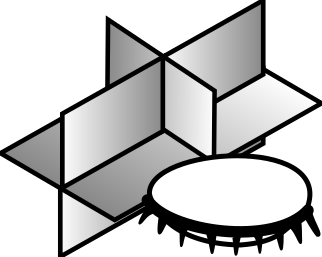
\includegraphics[width=0.7cm]{../../frontend/rsc/hide_planes} &
\textbf{Hide Crosshair}: Crosshair is hidden in planar views.\\
\hline
 & %No icon
\textbf{Taxonomy Selector}: Some tools may require the user to specify a
taxonomy label to be applied when segmentations are created.\\
\hline

\includegraphics[width=0.7cm]{../../frontend/rsc/removeSeg} &
\textbf{Delete Segmentation}: Deletes segmentations by clicking on them on one of the planar views.\\
\hline
\end{tabular}

\subsection{Channel Explorer}
Allows the user to individually toggle the visibility of each channel using a toogle button
located next to the channel's name whose function is similar of that described in the
general-purpose tools section.

\begin{figure}[H]
\centering
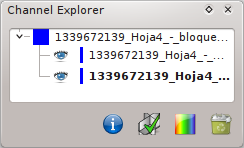
\includegraphics{fig/ChannelExplorer}
\caption{Channel explorer widget.}
\end{figure}

\begin{tabular}{| m{1.3cm} | m{12cm} |}
\hline
\textbf{Button} & \textbf{Description}\\
\hline
 & \textbf{Spacing Information}: Modify channel's spacing.\\
\hline

\includegraphics[width=0.7cm]{../../frontend/rsc/activeChannel} &
\textbf{Activate Channel}: Mark selected channel as active channel. Operations
are always applied to the active channel independently whether they are visible
or not.\\
\hline

\includegraphics[width=0.7cm]{../../frontend/rsc/rainbow} &
\textbf{Change Stain}: Display stain color selector for selected channel.\\
\hline

\includegraphics[width=0.7cm]{../../frontend/rsc/trash-full} &
\textbf{Unload Channel}: Unload current channel from \espina. The channel itself
is not modified nor deleted from disk.\\
\hline
\end{tabular}
\vspace{0.3cm}

\subsection{Taxonomy Explorer}

\begin{figure}[H]
\centering
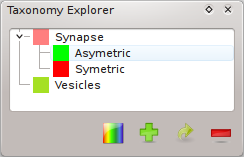
\includegraphics{fig/TaxonomyExplorer}
\caption{Taxonomy explorer widget.}
\end{figure}

\begin{tabular}{| m{1.3cm} | m{12cm} |}
\hline
\textbf{Button} & \textbf{Description}\\
\hline

\includegraphics[width=0.7cm]{../../frontend/rsc/rainbow} &
\textbf{Change Color}: Display taxonomy color selector for selected taxonomy.\\
\hline

\includegraphics[width=0.7cm]{../../frontend/rsc/create_node} &
\textbf{Add Taxonomy}: Create a new segmentation at the same level than the
selected one.\\
\hline

\includegraphics[width=0.7cm]{../../frontend/rsc/create_subnode} &
\textbf{Add SubTaxonomy}: Create a new segmentation as a child of the selected
one.\\
\hline

\includegraphics[width=0.7cm]{../../frontend/rsc/remove} &
\textbf{Delete Taxonomy}: Delete selected taxonomy.\\
\hline
\end{tabular}
\vspace{0.3cm}

\subsection{Segmentation Explorer}
Allows the user to individually toggle the visibility of each segmentation using a toogle button
located next to the segmentation's name whose function is similar of that described in the
general-purpose tools section.
\begin{figure}[H]
\centering
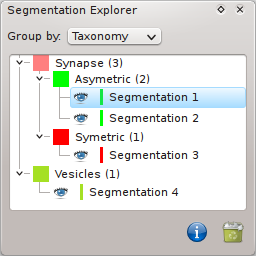
\includegraphics{fig/SegmentationExplorer}
\caption{Segmentation explorer widget.}
\end{figure}

\begin{tabular}{| m{1.3cm} | m{12cm} |}
\hline
\textbf{Button} & \textbf{Description}\\
\hline
 & %No icon
\textbf{Segmentation Information}: Open the segmentation inspectors for the
selected segmentations.\\
\hline

\includegraphics[width=0.7cm]{../../frontend/rsc/trash-full} &
\textbf{Delete Segmentation}: Delete selected segmentations.\\
\hline
\end{tabular}
\vspace{0.3cm}

\subsubsection{Segmentation Inspector}

Window composed of several widgets:
\begin{itemize}
\item a three-dimensional view
\item a filter inspector 
\item a data view
\end{itemize}
These widgets contain information about a single segmentation.

\begin{figure}[H]
\centering
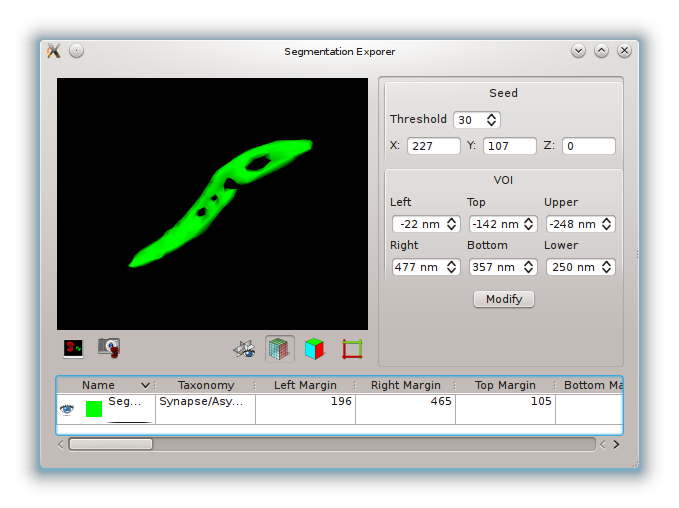
\includegraphics[width=\linewidth]{fig/SegmentationInspector}
\caption{Segmentation inspector widget.}
\end{figure}

For more specific information, please refer to the corresponding section.

\subsection{Volume Of Interest}

It's a volume to limit the effect of other tools, so the tool algorithm will not
go farther than the boundaries that define the volume.\\
To use it, just click on the toolbar button an then left click on the center of
the view area you want to place the volume of interest. Once the volume has been
placed the user can modify it's dimensions by clicking and dragging on the edges.\\
The user can define no more than one volume of interest at a given time. 

\vspace{0.3cm}
\begin{tabular}{| m{1.3cm} | m{12cm} |}
\hline
\textbf{Button} & \textbf{Description}\\
\hline

\includegraphics[width=0.7cm]{../../frontend/toolbar/voi/rsc/roi} &
\textbf{Rectangular Cuboid}: Define an axis aligned rectangular cuboid as volume
of interest.\\
\hline
\end{tabular}


\subsection{Seed Grow Segmentation}

This tool provides a semi-automated segmentation algorithm. Select a voxel
belonging to the object being segmented. A new segmentation will be createad
including all voxel which are equivalent (in gray scale values) to the selected
one, the seed.\\
If you have defined your own ``volume of interest'', then that is used instead of
the default one when applying the algorithm. The volume of interest will limit the
effect of the algorithm to the space enclosed within the volume.\\

\begin{figure}[H]
\centering

\includegraphics{fig/SeedGrowSegmentation}
\caption{Seed grow toolbar.}
\end{figure}
\vspace{0.3cm}

\begin{tabular}{| m{1.3cm} | m{12cm} |}
\hline
\textbf{Button} & \textbf{Description}\\
\hline
& %No icon
\textbf{Threshold}: Gray scale difference admisible to consider a voxel equal to
the one selected as seed. \\
\hline
& %No icon
\textbf{Default VOI}: Determine whether or not a rectangular volume of interest
centered on the selection point is applied.\\
\hline

\includegraphics[width=0.7cm]{../../frontend/toolbar/seedgrow/rsc/pixelSelector} &
\textbf{Pixel Selector}: Create a new segmentation using the voxel under the
cursor as seed for the Seed Grow Algorithm.\\
\hline

\includegraphics[width=0.7cm]{../../frontend/toolbar/seedgrow/rsc/bestPixelSelector} &
\textbf{Best Pixel Selector}: Create a new segmentation using the best voxel
,within the neighborhood of the voxel under the cursor, as seed for the Seed
Grow Algorithm. \\
\hline
\end{tabular}

\vspace{0.3cm}
\begin{bclogo}[couleur = yellow!33, logo= \bcbook]
{Tip} Use Ctrl+Wheel to change threshold while any selector is active. 
\end{bclogo}
\vspace{0.3cm}

Best voxel is defined in terms of gray scale similarity with a
reference gray scale value. The reference value can be configured at Seed Grow
Segmentation settings panel.\\

\subsubsection{Filter Inspector}
The filter inspector shows relevant information about the filter that created the segmentation,
therefore the information shown is dependent on the filter or plugin filter used.

\begin{figure}[H]
\centering
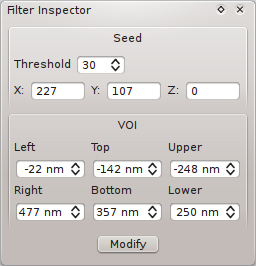
\includegraphics{fig/SeedGrowSegmentationFilterInspector}
\caption{Filter inspector widget showing the information of a seed grow filter.}
\end{figure}



%\section{Edition}

Segmentation tools, even if they are semi-automatic, need to be retouched in order to improve some analitical results.


%\section{Analysis}




%\bibliographystyle{alpha}
%\bibliography{rapport-mosig}

%\newpage

%\appendix

%\input{variables.tex}

%\input{architecture.tex}

%\input{coax_environment.tex}


\end{document}
